\documentclass{article}[12pt]

% useful packages
\usepackage{titlesec}
\usepackage{fullpage}
\usepackage{amsmath,amssymb,amsthm,amsfonts}
\usepackage{graphicx}
\usepackage{enumerate}
\usepackage{algorithm,algorithmic}
\usepackage{xcolor}
\usepackage{bbm}
\usepackage{url}
\usepackage{hyperref}

% theorem type environments
\newtheorem{thm}{Theorem}
\newtheorem{prop}{Proposition}
\newtheorem{lemma}{Lemma}
\newtheorem{cor}{Corollary}
\newtheorem{defn}{Definition}
\newtheorem{assump}{Assumption}
\newtheorem{example}{Example}
\newtheorem{conjecture}{Conjecture}

% frequently used symbols
\newcommand{\bE}{\mathbb{E}}
\newcommand{\bP}{\mathbb{P}}
\newcommand{\bQ}{\mathbb{Q}}
\newcommand{\bR}{\mathbb{R}}
\newcommand{\bS}{\mathbb{S}}
\newcommand{\bN}{\mathbb{N}}
\newcommand{\bZ}{\mathbb{Z}}
\newcommand{\sC}{{\mathcal C}} 
\newcommand{\sD}{{\mathcal D}} 
\newcommand{\sE}{{\mathcal E}} 
\newcommand{\sF}{{\mathcal F}} 
\newcommand{\sL}{{\mathcal L}} 
\newcommand{\sH}{{\mathcal H}} 
\newcommand{\sN}{{\mathcal N}} 
\newcommand{\sO}{{\mathcal O}} 
\newcommand{\sP}{{\mathcal P}} 
\newcommand{\sR}{{\mathcal R}} 
\newcommand{\sS}{{\mathcal S}}
\newcommand{\sU}{{\mathcal U}} 
\newcommand{\sX}{{\mathcal X}} 
\newcommand{\sY}{{\mathcal Y}} 
\newcommand{\sZ}{{\mathcal Z}}

% operators
\newcommand{\sign}{\mathop{\mathrm{sign}}}
\newcommand{\supp}{\mathop{\mathrm{supp}}} % support
\newcommand{\argmin}{\operatornamewithlimits{arg\ min}}
\newcommand{\argmax}{\operatornamewithlimits{arg\ max}}
\newcommand{\dist}{\operatorname{dist}}
\newcommand{\tr}{\text{tr}}
\newcommand{\vecop}{\text{vec}}
\newcommand{\st}{\operatorname{s.t.}}
\newcommand{\cut}{\setminus}
\newcommand{\ind}[1]{\mathbbm{1}\left\{#1\right\}} 
\newcommand{\given}{\ | \ }

% grouping operators
\newcommand{\brac}[1]{\left[#1\right]}
\newcommand{\set}[1]{\left\{#1\right\}}
\newcommand{\abs}[1]{\left\lvert #1 \right\rvert}
\newcommand{\paren}[1]{\left(#1\right)}
\newcommand{\norm}[1]{\left\|#1\right\|}
\newcommand{\ip}[2]{\left\langle #1,#2 \right\rangle}

% code commands
\newcommand{\matlab}{\textsc{Matlab }}
\newcommand{\python}{\textsc{Python }}
\newcommand{\todo}[1]{\textcolor{red}{#1}}

% header command
\newcommand{\project}[3]{
    \pagestyle{myheadings}
    \thispagestyle{plain}
    \newpage
    \setcounter{page}{1}
    \setlength{\headsep}{10mm}
    \noindent
    \begin{center}
    \framebox{
        \vbox{\vspace{2mm}
            \hbox to 6.28in { {\bf EE 519: Deep Learning Theory \& Fundamentals
            \hfill Spring \the\year} }
        \vspace{4mm}
        \hbox to 6.28in { {\Large \hfill Mini Project #3 \hfill} }
        \vspace{2mm}
        \hbox to 6.28in { \Large \hfill Due: #2, 11:59PM PT \hfill }
        \vspace{2mm}
        \hbox to 6.28in { {\it Student Name: #3} \hfill {\it Instructor Name: John Lipor}}
        \vspace{2mm}}
   }
   \end{center}
   \markboth{Mini Project #1}{Mini Project #1}
   \vspace*{4mm}
}

\begin{document}

% PUT YOUR NAME BELOW WHERE I HAVE \X
\project{1}{April 28, \the\year}{Andy Franck}
% PUT YOUR NAME ABOVE WHERE I HAVE \X

\section*{Problem Description}

The objective of this project is to train a multi-output convolutional neural network capable of accurate calculating both the horizontal and vertical diameter of an eyeball in an ultrasound image. After predicting, the model will be studied using guided backpropogation to determine what the trained model is used to make its predictions. The model will be trained on 100 ultrasound images of eyeballs, each with a manually labeled horizontal and vertical diameter.\\
\indent
Because of the nature of the image, the model may be able to make fairly accurate predictions even with the limited data size. This report aims to maximise the performance of the model by utilizing shared layers that branch off later into the model. This will allow the model to learn more general features of the image, and then use those features to make more accurate predictions.\\
\indent
Although basic in scope, the goal of this project is to make steps towards a more advanced method of pathology detection in ultrasound images. Ideally, this project would be the start of a larger project that would be able to determine more complex pathologies from ultrasound images, such as other tissues that are not visible through other methods of analysis.

\section*{Exploratory Data Analysis}

Because of the nature of the data, it was not necessary to perform much data analysis. It was easy to load directly from the files, and straightforward to work with through both the PyTorch and Numpy libraries. To begin, the ultrasound images were noted to have considerable area that was not useful for training. To fix this, the ultrasound images were cropped by 20\% to reduce unnecessary data. Because all of the eyeballs were taken in the center of the screen, and was considerable black space on the surrounding area, it was simple to crop the images without losing any useful data:\\

\begin{center}
    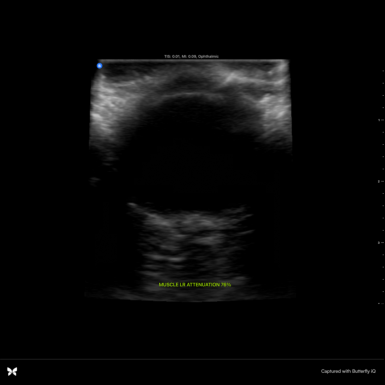
\includegraphics[width=0.3\textwidth]{images/uncropped.png}
    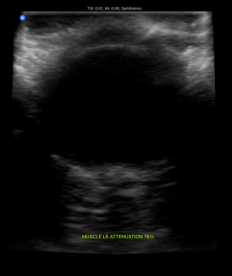
\includegraphics[width=0.3\textwidth]{images/cropped.png}\\
    \textit{Figure 1: Uncropped (left) and cropped (right) ultrasound images.}
\end{center}

\indent
Besides basic cropping, the data was also normalized to be between 0 and 1. This was done by dividing each pixel by 255, the maximum value of a pixel. This was done to make the data easier to work with, and to make the model more robust to changes in the data. \\

\indent
Finally, the labels were inspected to check data ranges, values, and distributions. The following are box and whisker plots of both the horizontal and vertical labels. It is clear from the picture that there are not many outliers, so no modifications were made to the labels.\\

\begin{center}
    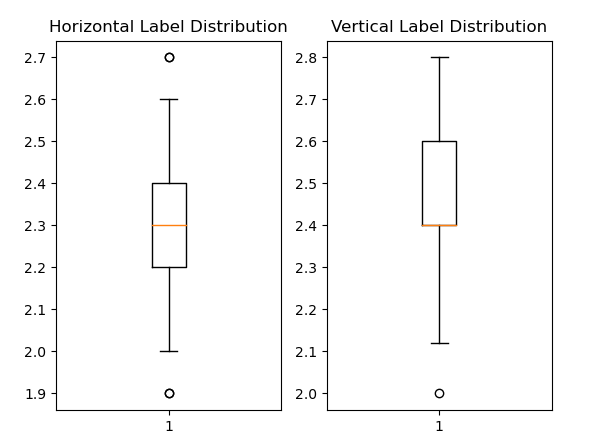
\includegraphics[width=0.7\textwidth]{images/label_distribution.png}\\
    \textit{Figure 2: Box and whisker plots of the horizontal and vertical labels.}
\end{center}


\section*{Challenges}

The largest challenge for this project was determining how many shared and seperate layers to use in the neural network model. Optuna was applied to the model however it was not able to find any significant improvements to the model, so it was discarded. Instead, the model was manually tuned to find the best combination of shared and seperate layers.\\
\indent
A dataset class was also made to load data properly into the dataloader with both y labels. This was done by creating a custom dataset class that would load the data and labels, and then return both the image and the labels. This was then passed into the dataloader, which was able to load the data into the model.\\
\indent
Additionally, it was difficult to determine exactly how accurate the model was predicting, since it is a standard regression problem. It was determined that if the prediction was truncated to the nearest hundreth, then it was a correct prediction.\\
\indent
Finally, the guided bkacpropogation analysis proved very difficult to implement. After adding hooks for the ReLU layers in the model, the analysis was subject to both exploding and vanishing gradients. Fortunately, this was solved by utilizing a different method to calculate the saliency maps without directly hooking the ReLU functions. \cite{saliency}

\section*{Approach}

The intial step in developmen involved creating a baseline Network in Network model with two outputs and all shared layers to get a baseline accuracy. The model implemented both batch normalization and dropout layers into the model based on the discoveries from the previous geothermal energy project. This model was used to make sure all data was being loaded properly, training was working as intended, and to establish a learning baseline to be build upon.\\

\begin{center}
    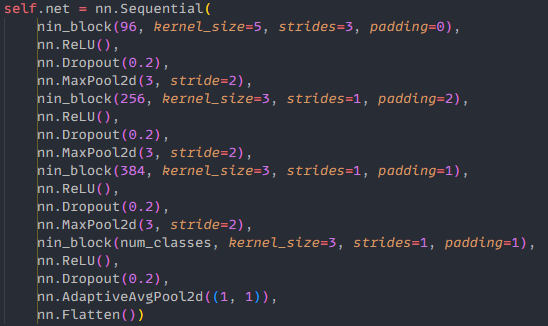
\includegraphics[width=0.6\textwidth]{images/baseline_model.png}\\
    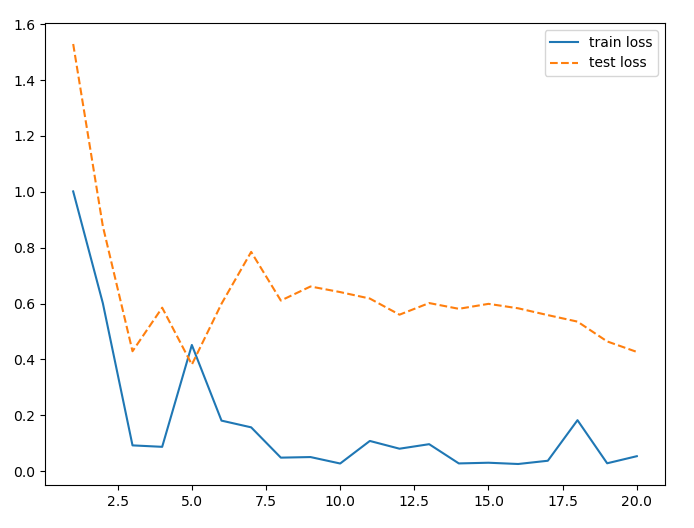
\includegraphics[width=0.6\textwidth]{images/baseline_model_graph.png}\\
    \textit{Figure 3: Baseline model architecture and loss graph.}
\end{center}

The model did not appear to be learning very well. Two methods were utilized to improve the performance of the model.\\
\indent
To artifically increase the data size, image augmentation was utilized via the torchvision.transforms library \cite{transforms}. This library allows for the creation of a transform object that can be applied to a dataset. The transform object contained both random flips and gaussian noise. The transform was applied after loading each batch at the start of the training loop, so that each batch was augmented differently.\\
\indent
Secondly, the model was modified to utilize both shared and seperate layers. This was done by taking the last two Network in Network layers and splitting them into a different Sequential object. This allowed for the model to learn more general features of the image, and then use those features to make more accurate predictions for both the horizontal and general diameters.\\

\begin{center}
    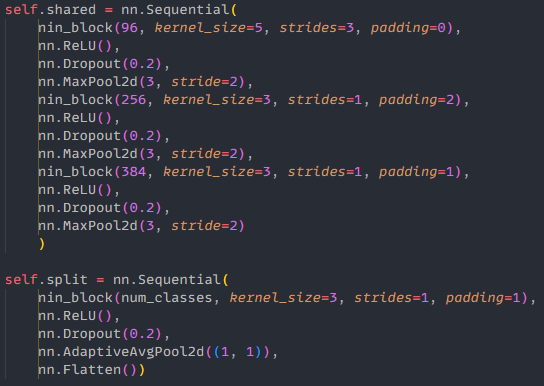
\includegraphics[width=0.6\textwidth]{images/final_model.png}\\
    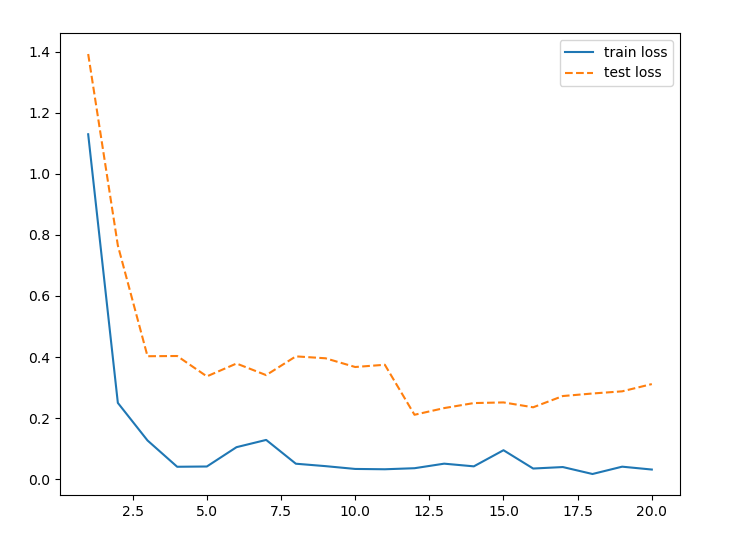
\includegraphics[width=0.65\textwidth]{images/final_model_graph.png}\\
    \textit{Figure 3: Updated model architecture and loss graph.}
\end{center}

Saliency maps of the model were generated using guided backpropogation, following the tutorial \cite{saliency} and \cite{backprop}. Originally, a hook was added to every ReLU activation layer in the network, and then the model was run on a single image. The gradients were then calculated at the output layer with respect to the input image. However, this method resulted in many gradient values equal to zero, so a modification was made following \cite{saliency} to calculate the gradients without directly hooking the ReLU layers.\\

\section*{Evaluation and Summary}


\section*{What I Learned}

This project was excellent practice for experimenting with more in-depth models. Data management and EDA were both very straightforward in this project, which allowed for more time to work on optimizing model parameters and layers in a multi-output format. \\
\indent
Additionally, now having some basic experience with image augmentation methods, it was interesting to discover more advanced methods to inflate the dataset. This was not particularly important for the project due to how quickly the model learned, however it was still interesting to learn about.\\
\indent
Finally, this projects use of saliency maps without classification was an interesting twist. Because it is difficult to determine a "correct" prediction, the nature of the maps and their usefulness was different than in previous projects. It was interesting to see how the maps were able to highlight the features of the image that the model was using to make its predictions, even without a classification task.\\

\bibliographystyle{IEEEtran}
\bibliography{bibliography}

\end{document}